\documentclass[12pt,a4paper]{article}
% !TEX program = xelatex
\usepackage[utf8]{inputenc}
\usepackage[T1]{fontenc}
\usepackage[finnish]{babel}
\usepackage[utf8]{inputenc}
\usepackage{graphicx}
\usepackage{titling}
\usepackage{titlesec}
\usepackage{booktabs}
\usepackage{fancyhdr}
\usepackage{lipsum}
\usepackage{comment, mdframed}
\usepackage{enumitem}
\usepackage{xcolor}
\usepackage{longtable}
%\usepackage{cite}
\usepackage{pgfgantt}
\usepackage{amsmath, amssymb}
\usepackage{tikz}
\usepackage[margin=1in]{geometry}
\usepackage[backend=biber, style=numeric]{biblatex}
%\usepackage{hyperref}
\usepackage{bookmark}
\usepackage{enumitem}
\usepackage{amsmath}
\usepackage{listings}
\lstset{language=Python, basicstyle=\ttfamily\small, breaklines=true,columns=fullflexible}
\lstset{escapeinside={(*@}{@*)}}
\usepackage{fontspec}
\setmainfont{Arial}
\newfontfamily\stylishfont{Noteworthy}
%\newfontfamily\stylishfont{Zapfino}
%\addbibresource{references.bib}
\usetikzlibrary{calc}
\usepackage{xcolor}

\lstdefinestyle{pidstyle}{
    basicstyle=\ttfamily\footnotesize,
    breaklines=true,
    escapechar=\#, % Define escape character for inline LaTeX commands
    linewidth=\textwidth,
    basicstyle=\ttfamily\scriptsize
}

\renewcommand{\maketitle}{%
  \begin{leftmark}
    \vspace*{\baselineskip} % Add a bit of vertical space

%    \includegraphics[width=4cm]{example-image-a} % Add an image before the title. you will need to replace the image path with your own

%    \vspace{0.5cm} % Add vertical space before title

    \textbf{\fontsize{18}{36}\selectfont \thetitle} % Font Size and Bold Title

     \vspace{0.05cm} % Add vertical space before subtitle
%    \textit{\Large \theauthor}  % Subtitle / Author
    \vspace{\baselineskip} % Add vertical space after subtitle
     \rule{\textwidth}{0.4pt} % Add a horizontal line

   \end{leftmark}
%    \thispagestyle{empty} % Prevent header/footer on the title page
}


% Section Formatting
\titleformat{\section}
  {\normalfont\fontsize{18}{22}\bfseries} % Font and style
  {\thesection}         % Section number
  {1em}                   % Horizontal space after section number
  {}                     % Code before the section name
  []                     % Code after the section name

\titleformat{\subsection}
  {\normalfont\fontsize{14}{18}\bfseries} % Font and style
  {\thesubsection}         % Subsection number
  {1em}                   % Horizontal space after subsection number
  {}                     % Code before the subsection name
  []                     % Code after the subsection name

\setlength{\parindent}{0pt}

\title{Computing platforms (Spring 2025)\newline
week 6}
\author{Juha-Pekka Heikkilä}



\pagestyle{fancy}
\fancyhf{}

\renewcommand{\headrulewidth}{0pt}

\newcommand{\footerline}{\makebox[\textwidth]{\hrulefill}}

\newcommand{\footercontent}{%
    \begin{tabular}{@{}l@{}}
        \footerline \\
        \leftmark \hfill \rlap{\thepage}
    \end{tabular}
}

\fancyfoot[C]{\footercontent}


\newcommand{\exercise}[1]{
    \section*{Tehtävä #1}
    \markboth{Tehtävä #1}{}
}

\addtolength{\hoffset}{-1.75cm}
\addtolength{\textwidth}{3.5cm}
%\addtolength{\voffset}{-3cm}
%\addtolength{\textheight}{6cm}
%\setlength{\parindent}{0pt}



% (a), (b), (c)
\newlist{kohta}{enumerate}{1}
\setlist[kohta,1]{
  label=\textbf{\makebox[1cm][l]{\Huge\text{(\stylishfont\alph*)}}},
  leftmargin=!,
  labelindent=0pt
}

% (1), (2), (3)
\newlist{alakohta}{enumerate}{1}
\setlist[alakohta,1]{
  label=\textbf{\makebox[1cm][l]{\Large\text{(\arabic*)}}},
  leftmargin=!,
  labelindent=0pt
}

% termi: selitys
\newlist{kuvaus}{description}{1}
\setlist[kuvaus]{%
  font=\bfseries\stylishfont,
  labelsep=0.5cm,
  leftmargin=2.5cm,
  style=nextline
}

\newcommand{\korostus}[2][yellow]{\colorbox{#1}{\strut #2}}
%\korostus{Yksi kirjoittaja on jo sisällä}
%\korostus[red]{Lukijan täytyy odottaa jos kirjoittajia on paikalla}
%\korostus[orange]{Tämä osa ei ole suoritettavissa}


\newcommand{\evalslantti}[4][-12]{%
%  \left. #2 \,\right|% ei indeksejä tähän
  \mkern-10mu\raisebox{0pt}[0pt][0pt]{\rotatebox{#1}{$\Big|$}}% vinoviiva päälle
  \mkern3mu{}_{\!#3}^{\!#4}% arvot viivan oikealle puolelle
}


\newcommand{\evalraise}{1.2ex}
\newcommand{\evallow}{1.2ex}

% vino eval-viiva, arvot oikealla (oletus: -12)
% \evalslant[asteet]{lauseke}{ala}{yla}
\newcommand{\evalslant}[4][-12]{%
  \left. #2 \,\right.%
  \mkern-10mu\raisebox{0pt}[0pt][0pt]{\rotatebox{#1}{$\Big|$}}%
  \mkern2mu{}^{\raisebox{\evalraise}{$\scriptstyle #4$}}_{\raisebox{-\evallow}{$\scriptstyle #3$}}%
}



% vino eval-viiva ENNEN lauseketta
% \evalslantpre[asteet]{lauseke}{ala}{yla}
\newcommand{\evalslantpre}[4][-12]{%
  % viiva ja rajat
  \raisebox{0pt}[0pt][0pt]{\rotatebox{#1}{$\Big|$}}%
  \mkern2mu{}^{\raisebox{\evalraise}{$\scriptstyle #4$}}_{\raisebox{-\evallow}{$\scriptstyle #3$}}%
  % itse lauseke
  \mkern4mu\left. #2 \right.%
}


\DeclareMathOperator{\Var}{Var}
\DeclareMathOperator{\Cov}{Cov}
\DeclareMathOperator{\Corr}{Corr}

\newcommand{\set}[1]{\left\{\,#1\,\right\}}
\newcommand{\abs}[1]{\lvert#1\rvert}

\newcommand{\N}{\mathbb{N}}
\newcommand{\Pot}{{\cal P}}

\newcommand{\rma}{\mathrm{a}}
\newcommand{\rmb}{\mathrm{b}}
\newcommand{\rmc}{\mathrm{c}}

\title{TKT20005 Laskennan mallit Viikko2}
\date{}

\begin{document}

\maketitle

\exercise{1 Perustermejä.}
Selitä omin sanoin seuraavat termit: merkki, aakkosto, merkkijono, formaali kieli. Anna esimerkki merkistä, aakkostosta, merkkijonosta ja formaalista kielestä.

\paragraph{Merkki} on symboli mikä on aakkoston alkio. Esimerkiksi 0, 1, HiiriVasen, tkt, mat.
\paragraph{Aakkosto} on mikä tahansa äärellinen joukko. Esim. ASCII merkistö, {R, G, B, A}
\paragraph{Merkkijono} Aakkoston jono, äärellinen jono symboleita, Esim. 00010 on aakkoston $\Sigma_1$ merkkijono.
\paragraph{Formaali kieli} Formaali kieli A on sellainen sääntöjen joukko että sillä on tarkastaja V joka hyväksyy tai hylkää alkion.



\exercise{2 Joukko-opin merkinnät I.}
Kuvaile sanallisesti seuraavat joukot:
\begin{kohta}
\item $\set{2n+1\mid n\in\N}$ on parittomien luonnollisten lukujen joukko, esim 1, 3.
\item $\set{ww^{\cal R}\mid w\in\set{0,1}^\ast}$, missä 0 ja 1 ovat merkkejä. On palindromien joukko missä joukon jäsenet on parillisen pituisia. 0110, 011110
\item $\set{\rma^n\rmb^n\rmc^n\mid n\in\N}$, missä $\rma$, $\rmb$ ja $\rmc$ ovat merkkejä. On joukko missä on sama määrä a, b ja c merkkejä \epsilon, abc, aabbcc
\item $\set{u\in\Sigma^\ast\mid
\mbox{jollakin $v\in\Sigma^\ast$ pätee $uv=\mbox{\tt abrakadabra}$}}$,
missä $\Sigma=\set{\mbox{\tt a},\ldots,\mbox{\tt z}}$. On alusta purkaen sanan abrakadabra loppuosat. abrakadabra, brakadabra, rakadabra
\end{kohta}
Anna lisäksi kustakin joukosta kaksi esimerkkiä joukkoon kuuluvista
alkioista.




\pagebreak
\exercise{3 Joukko-opin merkinnät II.}
Esitä tehtävän~2 tyylistä joukkomerkintää
käyttäen seuraavat joukot:
\begin{kohta}
\item
aakkoston $\set{\mathrm{a},\mathrm{b},\mathrm{c},\mathrm{d}}$
palindromit
(merkkijonot, jotka ovat samoja myös lopusta alkuun luettuina.)\\

$\set{w \in \set{a,b,c,d}^* | w = w^R } $
\item
kolmella jaolliset luonnolliset luvut\\

$\set{w \in \mathbb{N} | w\, mod 3 = 0 } $
\item
aakkoston $\set{0,1}$ merkkijonot, joissa kaikki nollat ovat
ennen ykkösiä\\

$\set{{0^n 1^m}|n, m \in \N } $
\item
aakkoston $\set{\rma,\rmb}$ merkkijonot, jotka sisältävät
osamerkkijonon $\mathrm{bab}$.\\

$\set{wbabx \mid w, x \in \set{a, b}^*  } $\\

bab, abab, baba, bbab, babb, aabab, ababa, ababb, babaa, babab


\end{kohta}
Luettele lisäksi (d)-kohdan kielen kymmenen ensimmäistä
merkkijonoa lyhytaakkosjärjestyksessä (shortlex).




\pagebreak
\exercise{4 Äärellisen automaatin määritelmä ja sen tunnistama kieli.}
Tässä tehtävässä harjoitellaan äärellisen automaatin tilakaavion piirtämistä ja tulkintaa.\\

Olkoon $M=(\set{q_0,q_1,q_2},\set{0,1},\delta,q_0,\set{q_2})$,
missä $\delta$ on seuraava:
\begin{center}
\begin{tabular}{c|cc}
& 0 & 1\\\hline
$q_0$ & $q_1$ & $q_0$\\
$q_1$ & $q_2$ & $q_0$\\
$q_2$ & $q_2$ & $q_2$
\end{tabular}
\end{center}
\begin{kohta}
\item Esitä automaatti $M$ tilakaaviona.
\begin{figure}[h]
  \centering
  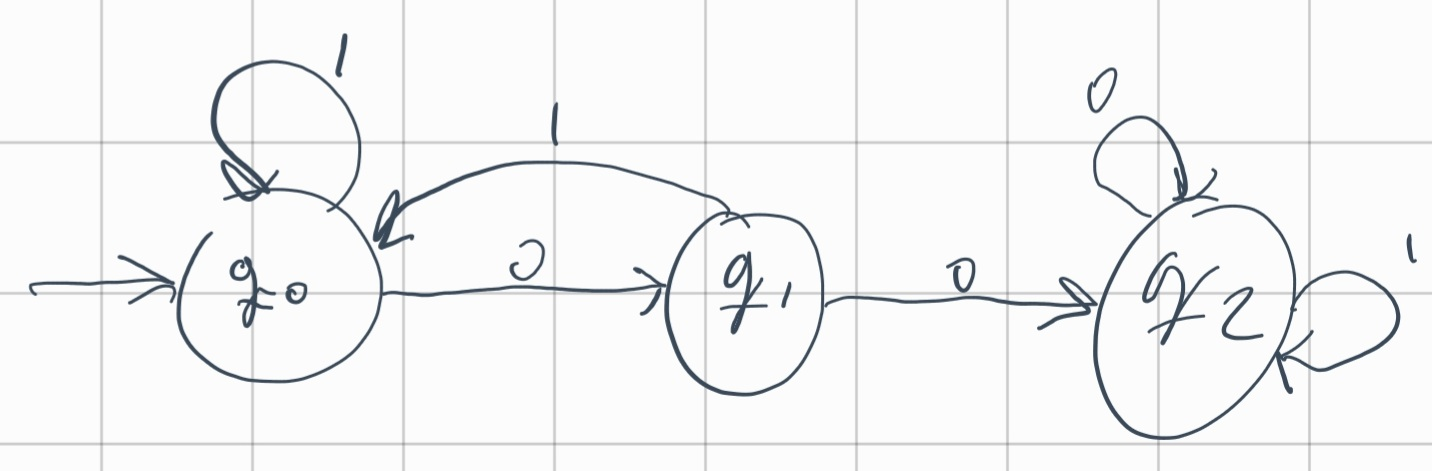
\includegraphics[width=.8\textwidth]{viikko2tehtävä4.jpg}
\end{figure}
\item Luettele järjestyksessä tilat, joissa automaatti käy syötteellä 10101010 ja syötteellä 010011. Hyväksyykö vai hylkääkö automaatti syötteen?\\

q0, q0, q1, q0, q1, q0, q1, q0, q1\\

automaatti hylkää syötteen koska q1 ei ole sallittu tila.\\

q0, q1, q0, q1, q2, q2, q2\\

automaatti hyväksyy söytteen.

\item Kuvaile sanallisesti automaatin tunnistama kieli.\\

Eli miten q2 pääsee? Vaikuttaisi että q0->q1->q2 tarvitaan
kaksi peräkkäistä nollaa. Eli automaatti tunnistaa syötteet missä on
kaksi peräkkäistä nollaa.
\end{kohta}



\pagebreak
\exercise{5 Lisäharjoitusta äärellisen automaatin tunnistaman
kielen kuvailuun.}

\paragraph{Vasen automaatti} kuvaa kieltä joka alkaa a:lla
ja päättyy a:han. Merkkijono vuorottelee merkkejä a,b,a,b,a.
Merkkijonon pituus on pariton ja parittomissa paikoissa on a.

Eli alkaa a:lla ja sitä seuraa nollasta ylöspäin kertaa ba.

\paragraph{Oikea automaatti} kuvaa kieltä mikä sisältää nollasta
ylöspäin kertaa 'ab' ja 'ba' merkkiyhdistelmiä.

\bigbreak



\pagebreak
\exercise{6 Formaalit kielet.}
Tässä tehtävässä opetellaan esittämään ja todistamaan argumentteja formaaleista kielistä.

Kieli $A$ on {\em rajoitettu}, jos sen merkkijonojen pituudet ovat
ylhäältä rajoitettuja, ts.\ jollain luonnollisella luvulla
$n\in\N$ pätee, että $\abs{w}\leq n$ kaikilla $w\in A$.

\begin{kohta}
\item % 1) Unioni
Pitääkö paikkansa, että kahden rajoitetun kielen $A$ ja $B$
yhdiste $A\cup B$ on aina rajoitettu? Todista väite tai anna vastaesimerkki.\\

Olkoon $A\subseteq \bigcup_{i=0}^{M}\Sigma^i$ ja $B\subseteq \bigcup_{i=0}^{N}\Sigma^i$\\

Silloin (lausetta 1.1 seuraten)

\[
A\cup B \;\subseteq\; \bigcup_{i=0}^{\max\{M,N\}} \Sigma^i
\]
joten kaikilla $w\in A\cup B$ pätee $|w|\le \max\{M,N\}$. Siis $A\cup B$ on rajoitettu.



\item % 2) Leikkaus
Pitääkö paikkansa, että kahden rajoitetun kielen $A$ ja $B$ leikkaus $A\cap B$ on rajoitettu? Todista väite tai anna vastaesimerkki.\\

Yllä määritellyillä M,N jos $w\in A\cap B$, niin $|w|\le M$ ja $|w|\le N$, joten
$|w|\le \min\{M,N\}$\\

Siis
\[
A\cap B \;\subseteq\; \bigcup_{i=0}^{\min\{M,N\}} \Sigma^i
\]
ja $A\cap B$ on rajoitettu



\item % 3) Iff äärellinen
Todista, että kieli on rajoitettu, jos ja vain jos se on
äärellinen (ts.\ sisältää tasan $m$ merkkijonoa jollain
luonnollisella luvulla $m\in\N$).\\

Jos L on rajoitettu, niin on N siten, että $|w|\le N$ kaikilla $w\in L$ \\

Silloin
\[
L \;\subseteq\; \Sigma^{\le N} \;:=\; \bigcup_{i=0}^{N}\Sigma^i
\]
Koska $\Sigma$ on äärellinen, jokainen $\Sigma^i$ on äärellinen ja äärellinen
unioni äärellisiä joukkoja on äärellinen, joten $\Sigma^{\le N}$ ja siten $L$ on äärellinen.

\end{kohta}


\end{document}